\documentclass[tikz,border=8pt]{standalone}
\usepackage[utf8]{inputenc}
\usepackage[OT4,plmath]{polski}
\usepackage{amsmath}
\usetikzlibrary{patterns}
\begin{document}
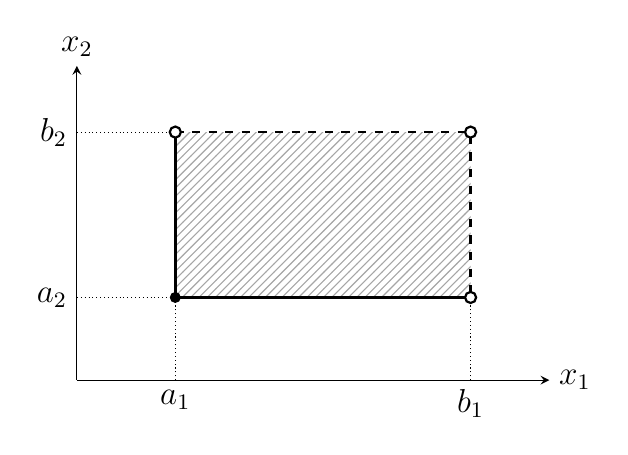
\begin{tikzpicture}[x=1.25cm,y=1.05cm,>=stealth,font=\large]
  \draw[->] (0,0)--(4.8,0) node[right] {$x_1$};
  \draw[->] (0,0)--(0,3.8) node[above] {$x_2$};
  \fill[pattern=north east lines,pattern color=black!35]
    (1,1) rectangle (4,3);
  \draw[very thick] (1,3)--(1,1)--(4,1);
  \draw[thick,dashed] (1,3)--(4,3)--(4,1);
  \foreach \x/\lab in {1/a_1,4/b_1} {
    \draw[densely dotted] (\x,0)--(\x,1);
    \node[below] at (\x,0) {$\lab$};
  }
  \foreach \y/\lab in {1/a_2,3/b_2} {
    \draw[densely dotted] (0,\y)--(1,\y);
    \node[left] at (0,\y) {$\lab$};
  }
  \fill (1,1) circle (2pt);
  \foreach \p in {(1,3),(4,3),(4,1)} {
    \draw[fill=white,thick] \p circle (2pt);
  }
\end{tikzpicture}
\end{document}
